\section{Introduction}

\begin{figure*}[h]
    \centering
    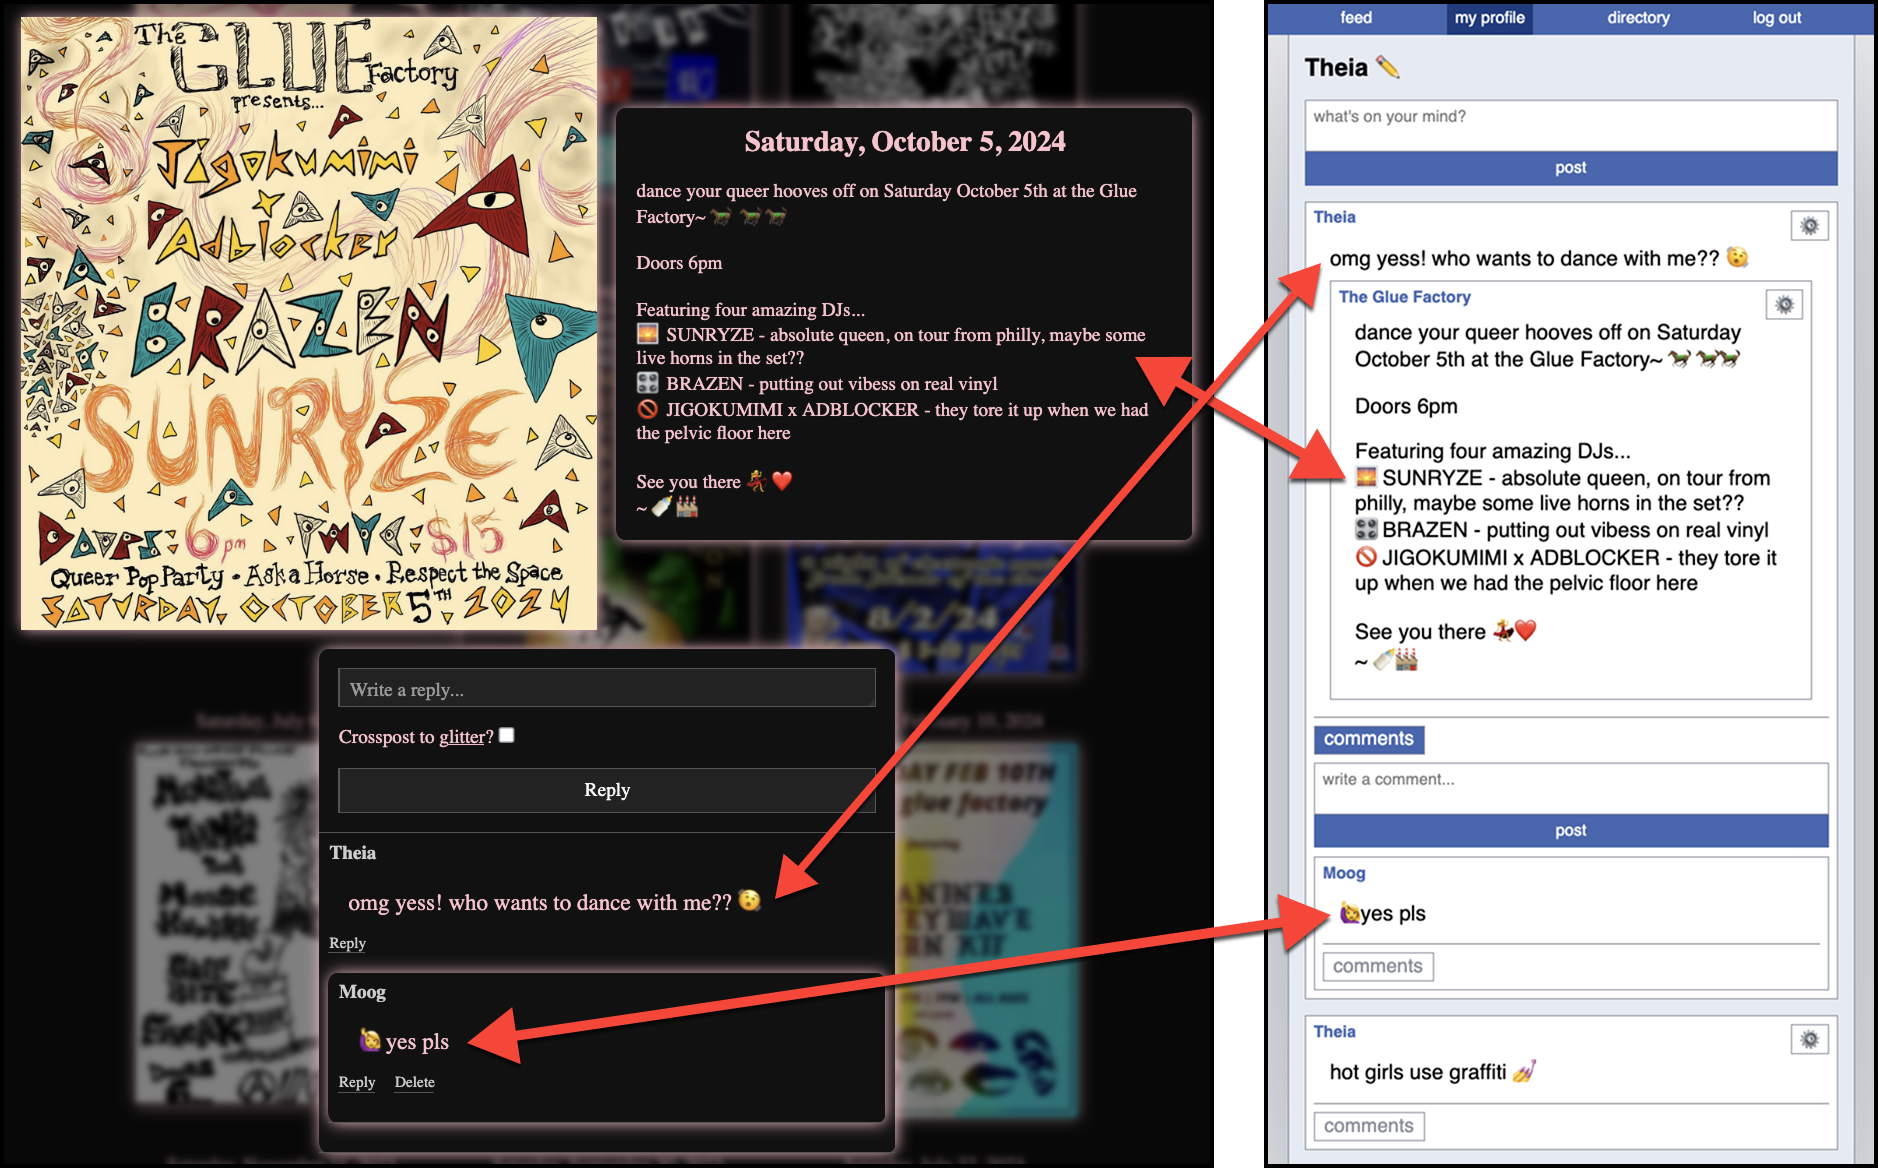
\includegraphics[width=\textwidth]{paper/figures/gloof-and-glitter.jpg}
    \caption{
    Interoperation between two applications built with Graffiti:
    The Glue Factory, an application operated by a venue to advertise their shows,
    and Glitter, a microblogging site.
    }
    \label{case-studies:fig:gloof-and-glitter}
\end{figure*}

Most social applications today are built like international airports,
designed to serve everyone, and soulless as a result.
Where are the online spaces that feel like
the unofficial skate park behind the grocery store,
the dance floor of a long-running nightclub,
or that one friend's living room?
% or that one friend's living room where you can always show up?
Where are those intentional community spaces that
are not meant for everyone,
but are \emph{everything} to the people
who collectively curate their aesthetic and social norms?

Their absence is partly because truly personalized social applications
%DK given the framing you are using here, I wonder if "social web sites" is better than "social applications" (or if you need to use both and explain why).   Your examples---the nightclib, the friend's living room (and also Gloof) feel like sites not apps.   Per my email, it may be useful or necessary to talk somewhere in the paper about the difference between sites (you go there to interact with a certain kind of contet pertinent to the site?) ad apps (you pull in content from all over to interact with?) and how with gradfiti there is't really a differece
are extremely difficult to build,
and partly because the great power of social media---its
ability to connect massive numbers of people---also
creates social pressure for everyone to use the same few applications.
% one of the powers of social media
% is that it is not limited by space or distance
% but this leads the question of "who" the community is
% that has control over this space.
% are extremely hard to build from scratch,
% both from technical expertise and the social challenge of building a user base.
% And modifying existing ones is not an option
% or modification requires either technical expertise
% or breaking away.


% Social applications today are like international airports:
% globalized and one-size-fits-all, devoid of any specific
% culture, purpose, meaning.
% What if instead they felt like intentional community
% spaces: that one friend's living room,

% Places with charachter, spoken, written into contracts,
% or spraypainted on the wall.

% Intentional community spaces
% What if instead they were like that one friend's living room,
% the dancefloor and a long-lived nightclub,
% the club, the punk house?

% Living in an intentional community,
% can control the arrangement of furniture, the

% or a cooperative house, perhaps you've had
% the chance to

% Consider the spaces you've loved to socialize in.
% % where had some of your favorite social experiences.
% Maybe it was that one friend's living room,
% or the park your kid plays at,
% % or your grandma's dining room table,
% or the dancefloor of a club.

% Instead, our the social spaces we inhabit online
% are built like international airports:
% globalized, one-size-fits-all designs
% devoid of any meaning.
% Why is there such a disconnect between the two?


% Now why do our online spaces instead feel like
% international airports: minimal, homogenized,
% one-size-fits-all.
% Now imagine that in an airport:
% globalized, just like all of our online spaces.


% globalized

% Why can't we choose from
% Why can we not build living rooms,
% or parks, or clubs?

% The decor, the arrangement of ,
% the social norms, spoken or otherwise,


% While the people, obviously do work,
% how was the space itself curated to
% fit their needs?

% had some of your favorite social experiences.
% Maybe it was around a bonfire,
% or at a neighborhood potluck,
% or on the dancefloor of a club,
% or in that one friend's living room.
% or at a party,
% or at a dinner table,
% Besides the people how did the space shape the experience?


% Bring in the details of that setting:
% the decor, the food, the social norms,
% the rituals.

% The arrangement of people and furniture,

% Then consider one of the small handful of online
% spaces we all inhabit. One-side-fits one.


% the dearest the social spaces you've frequented
% in the real world. Perhaps its that
% one's friends living room,
% a picnic bench after a round of soccer, or
% the dancefloor at a club.
% Consider all the details in those spaces that:
% the furniture, the lighting,

% Why then do we use a small handful online spaces that

% in those spaces and what sets them
% apart from all the other spaces you've visited.

% When then, do the social spaces we inhabit
% feel. Perhaps you can change the people you
% follow or some cursory settings, but then what?

% These visceral

% soccer games
% In all of them,

% Now consider the spaces online.
% While you might have control over who you follow,
% can you even change the color scheme?

% Why is there such a disconnect between the diverse
% autonomous spaces we inhabit in the real world,
% and the
% Part of the issue is the ``furniture'' of social applications
% is the features we interact with and rearranging it can be extremely
% challenging.
% Part of the issue is that, without space as a limiting factor,
% social spaces can grow large and people
% can get locked-in.


% There are millions of apps and billions of websites but
% most people socialize on a tiny handful of
% Today, most people's online social interactions are mediated
% by small handful of globalized, homogenized, one-size-fits-all applications.
% Why can't these applications feel more like
% that one friend's living room.
% A space where, over time,
% the furniture and the decor has slowly arranged itself
% to best suit the needs and preferences of its inhabitants,
% and social norms develop, sometimes written down,
% about acceptable behavior.


% the furniture has slowly arranged itself
% over years of intentional and decisions to best suit,
% mementos from, and norms.

% main street on a saturday night,

% Intimate, opinionated spaces where
% every aspect of their design is a reflection of the
% communities they serve and to some extent.


% or a neighborhood cook out.

% a community center,
% Spaces where every aspect, from the arrangement of the furniture,
% to the social norms, stated or not, is curated by that community.


% Why can't we personalize them, like our living rooms and social
% spaces where everything from the arrangement of the furniture,
% to the guest list, to the social norms can be created by the
% community that frequents it?

% In the real world opionated
% Why are they so different than our physical spaces,
% where every aspect from the arrangement of the furniture,
% to the guest-list, to the norms can be
% Why can't these applications be more like the social spaces?
% Where everything from the arrangement of the furniture,
% to the lighting, who is invited, what the norms are.

% in a social application requires signifigant technical expertise
% to introduce new social
% is quite complicated.
% But part of it is that online
% , without the requirement
% everyone flocks to where everyone already is, locking
% in to a particular experience.
% Part of it is that
% of digital applications requires signifigant technical expertise
% requires significant technical expertise,
% and partly because network effects pressure
% people to gather where their friends already are.

We present a system called \emph{Graffiti} that makes
building \emph{personalized} social applications
%and social sites with distinctive personalizities
more accessible,
while maintaining the interconnectedness that is special to social media.
We lay the foundation for developers to create a diverse ecosystem
of social applications
%and sites
with only client-side code and with minimal friction
to introducing new features,
% with relative ease, using only client-side code
% and with minimal friction to introducing new features,
while also ensuring that these applications \emph{interoperate},
allowing people to freely migrate between them without
losing their friends or data.
The types of social applications that can be built on the same set of Graffiti primitives range from analogs of Twitter to Facebook to Messenger to Slack to Goodreads to Pinterest to Wikipedia,
with plenty of room for entirely new creations.
%including social ``sites'' with distinctive personalities.

%DK intro should discuss "the wall"

\hl{%
Our goal of interoperability leads almost immediately
to the conclusion that a user's
social data---their posts, likes, friend lists, and so on---\emph{cannot}
be stored within any single application.
Instead, user data is stored on a collective infrastructure
that all applications can access (subject to access control)
and selectively present data from according to their individual designs.
}%

\hl{%
This application-infrastructure separation
is an interoperability mechanism similar to
those used by
ActivityPub~{\cite{activitypub}},
which underlies Mastodon,
and the AT Protocol~{\cite{bluesky}}, which underlies Bluesky.
However, these social protocols---primarily designed to support
Twitter-like networked interactions---are limited in the range of applications
and features they can support.
Some limitations stem from hardwired assumptions,
like per-``instance'' moderation in ActivityPub
or the public-only visibility of content in the AT Protocol.
Other capabilities are technically \emph{possible}
but require standing up custom servers or navigating
a slow and complex standardization process.
% to perform out-of-band interactions.
In contrast, Graffiti provides a simple yet minimally constraining
client-side \emph{application programming interface} (API)
upon which a much broader range of personalized applications can be built, all
without server code or bureaucracy.
}%

% To illustrate the ecosystem this enables,
% suppose a group of friends start out by using an Instagram-like application,
% but some get bored of the interface and so by using the copy-and-paste
% programming that used to be popular on MySpace~\cite{copypasteliteracy}
% they make a ``fork'' of the application.
% Not everyone switches, which is fine because posts show up in either,
% but those who do get sparkly animations, the ability to
% add a colored halo around posts (to reflect their aura that day),
% and the ability to mark pictures of friends that look extra cute---the pictured
% friend can add the photo to their Tinder-like profile with a click.

% a group of users start using a Discord like server
% but then, largely from copy-and-pasting bits of
% code from other sites, like MySpace, they make it personal
% with features like X and Y.
% Unfortunately, an argument splits the group up,
% rather than one group getting custody of the app,
% they can continue on with two seperate ``views''.
% One application becomes popular and the other stays
% between a small group of friends, continually adding
% new features.
%DK maybe a simpler story, where an artist posts a new video on her "youtube channel", and a fan who is following her sees that post in his "twitter feed" and forwards it over "whatsapp" to his friends who talk about it there for a while with the result that eventually one of the friends uses "whatsapp" to "reply to" the original video post and that "reply" shows up as a comment on the artist's video on "youtibe".   Focus on the dyamics of the content without too much backstory about the participants.

% To achieve our goals of maximum personalization and interoperability, the "communication core" of Graffiti is kept as minimal and generic as possible, responsible only for delivering content from users' applications that post to to users' applications that want to access it; it can almost be thought of as a social analogue of TCP/IP.   All \emph{interpretation} of the transported content is left to the pure-client applications that create and consume it.  The communication core is so minimal that it only delivers \emph{notifications} about user posts, while the actual content of the users' posts can be kept in whatever personal storage those users' wish to use, such as their dropbox directories.  This again maximizes user control.


A key challenge of Graffiti's design is to resolve
the \emph{tension} between personalization and interoperability.
Allowing applications to have different styling is
not a problem, but can an application with top-down
moderation interoperate with a democratically moderated one?
Is it possible for a small community forum to exist and
not get flooded by the rest of the ecosystem's traffic?
% a use
% applications have incompatible
% notions of reach or quiet posting
% a user posts from an application with
% ``quiet'' posting
% strict privacy settings,
% while they are viewed from an application with loose ones?
We resolve these questions respectively with two concepts: \emph{total reification},
where all social interactions
%---including upvotes, replies, shares, quotes, moderator deletions, blocks, and edits---
are first-class objects that
%are published as separate \emph{annotations} on underlying objects and
can be interpreted or ignored by different applications;
and \emph{channels}, which organize data contextually,
preventing a phenomenon called ``context collapse''~\cite{contextcollapse}.


% In Graffiti, yes. Our concept \emph{total reification}
% treats moderation, and in fact all social interactions,
% as first-class objects that can be interpreted
% or ignored by different applications.
% In this case, our \emph{channels} concept helps respect the wishes of the poster,
% maintaining their ``imagined audience'' and preventing context collapse.

Our design decisions are guided by a set of \emph{requirements}, outlined
in Section~\ref{requirements}, that primarily focus on the direct experience
of social application developers and the users of their applications,
both users of Graffiti as a whole.
\hl{%
We include one additional requirement that targets the indirect
effects that \emph{power} over the underlying infrastructure
can have on the user experience.
Specifically, we leave room for users to retain control over their data
via technologies like decentralization or encryption.
}%

\hl{%
Importantly, however, Graffiti is not shaped by a particular
means of achieving this distribution of power. This again contrasts Graffiti
with systems like ActivityPub and the AT Protocol,
which are inseparable from their decentralized architectures
and leak architectural details, like ``instances'' and ``relays,''
into their APIs.
Graffiti's API-first\footnote{
We reply to the provocation ``\emph{Protocols, Not Platforms}''~{\cite{protocolsnotplatforms}},
the rallying cry that sparked Bluesky~{\cite{bluesky_from_protocols}},
with the amendment, ``\emph{...but the API first!}''
} approach not only reduces complexity for
developers who simply want to make applications,
but also allows the infrastructure underneath
to update as both technologies and threats evolve.
In fact, the Graffiti API is designed so that multiple implementations can exist
\emph{in parallel} underneath it,
allowing for the incremental adoption of new technologies,
similar to the web's transition from HTTP to HTTPS.
}%
% We reply to the provocation ``\emph{Protocols, Not Platforms}''~\cite{protocolsnotplatforms},
% the rallying cry that sparked Bluesky\footnote{
% \url{https://bsky.app/profile/jay.bsky.team/post/3kkrxedmatv2p}
% },
% with the amendment, ``\emph{...but the API first!}''

After our requirements, we describe the Graffiti API,
first through high level concepts in Section~\ref{concepts},
then in detail in Section~\ref{api}.
Section~\ref{above-and-below} describes
the decentralized protocols we have built \emph{below} the API,
as well as the tooling we have developed \emph{above} the API
to build Graffiti applications with declarative and reactive programming.
In Section~\ref{case-studies},
we evaluate Graffiti through a series of case studies, demonstrating
how it is possible to build applications like Twitter, Messenger, and
Wikipedia, as well as novel applications on Graffiti, and how unusual
variants of all of these interoperate.
Finally, we wait until Section~\ref{related-work}
to continue exploring related work, by then with a more concrete
understanding of what we are relating to.

% Unforuntately, some of the social implications of our
% system, are left to another paper but we conclude
% with leading questions.

% s tools we've built above the API
% Section
% The requirements below are for our primary contribution, our \emph{API}. The design that meets these
% requirements is covered in the following
% We also outline a set of \emph{protocols} that implement the API in Section~\ref{protocols}, each with their own
% requirements and tradeoffs, but all of which can coexist.
% We have also built additional tools \emph{above} the API, to enable
% ``reactive'' programming and to make common designs easier
% We also provide different implementations \emph{below} the API
% involing communication \emph{protocols}.

% We work towards alleviating both of these problems.
% reducing the barrier to entry to making a wide variety of applications
% while also allowing for those applications to \emph{interoperate}
% with data smoothly flowing across them.
% We introduce Graffiti, a novel infrastructure that aims to make social media applications easier to create, change, and migrate between in the hope that the ecosystem of applications will evolve to be better for both individuals and society.

% The core of Graffiti is a generic API for publishing and discovering social data. The API is designed so that many different client applications can be built on top it simultaneously, allowing those apps to naturally interoperate so that content posted in one client can be read in another.

% Related systems, that allow for different frontends to be built on top of a shared social backend, bake design patterns into their APIs that limit the gamut of applications that can be built.
% For example, users can switch between different frontends for Mastodon and BlueSky, but they still follow the general microblogging design pattern: a feed of posts with likes and comments.

% Graffiti, on the other hand, is highly \emph{pluralistic} and can be used to create Twitter clones, but also clones of Reddit, Pinterest, Yelp, and Wikipedia, in addition to radically different designs.
% In particular,
% it allows for an evolving ``folksonomy'' of data types, the creation of social boundaries despite its interoperability, coexisting moderation policies, and allows data to be forgotten.

% We actualize the Graffiti API from ``above'' with a Typescript client library and a Vue.JS plugin that we use to build an array of example applications.
% makes it possible to build complete social applications using only front-end development tools on top of the generic Graffiti API.
%
% We actualize Graffiti API from ``below'' with a decentralized backend that implements API.
% In this implementation, users host their social data in a storage pods of their choice and a decentralized tracker tells clients which pods they should query to find relevant data.
% Together, the technology stack composed of the API, client side tools, and decentralized backend form the complete Graffiti infrastructure.

% Our analysis of Graffiti is primarily focused on the design of the API. The client side tools make it possible to build.

% Graffiti at its heart rellects a simple design: each user hosts their own content/posts on their own storage service such as Dropbox or Solid, partitioned into \emph{channels} intended for different audiences, and social client applications collect, organize, lnd present that content for users who want it.   A simple, scalable \emph{tracker} helps clients keep track of content they should collect.   Graffiti can be seen as an evolution of RSS feeds and readers, with added realtime notification and interaction capabilities to support social applications.

% [Add something about how the affordances of a system mirror cultural partices of communities (Black Twitter, distruted blackness) and can reinforce existing hierarchies (design justice)]

% Graffiti is generally a liberal system that prioritizes self determination
% over paternahism, however we present both centralized and decentralized implementations as different approaches to the trolley problem that pits the need for a central entity that can detect repugnant behavior (e.g. CSAM) against the values of privacy and free speech.

% Aside from this possible root-level filter for universally repugnant content,
% moderation is performed independently by different clients using annotations from the user or from user-selected third-parties to hide, flag, or demote unwanted content.
% Data is not limited to rigidly defined concepts like ``posts,'' ``replies,'' or ``likes;'' instead, clients can interpret data flexibly according to an evolving folksonomy.
% Users enjoy the ``right to be forgotten,'' and plausible deniability for their posts, unless they explicitly opt-in to third party signing services.
% One of the system's few enforced constraints aims to prevent context collapse~\cite{contextcollapse}, the flattening of multiple audiences, giving users a sense of ``place'' in an otherwise amorphous sea of data.

% To the extent possible, Graffiti is built upon existing infrastructure.
% In our decentralized implementation, users posts are hosted on their own cloud storage provider like Dropbox or Solid.  We connect these personal data stores together to form a global content discovery network using a tracker, a concept borrowed from BitTorrent.  The demands on the Graffiti tracker are minimal, making the system quite scalable.
% In both implementations, the data passing through the system is based on the Activity Vocabulary web standard.

% We developed a prototype Typescript library that connects to these backend components and exposes a simple API for frontend development. Additionally, we created created a Vue.JS plugin on top of the library that lets developers write entire social applications declaratively.

% We analyze Graffiti through a number of case study applications that demonstrate the ease of development, interoperability, and a diversity of possible application designs.
% We also discuss the system's performance at scale, its economics, its adoption, and its potential for abuse.

% Moderation actions are annotihns of data and can be interpretted as.
% The receiving client can then choose to display the data based on it's own moderation policies.

% , subject to three contraints.
% First, the producing and consuming clients must utilize a common \emph{context}, a mechanism designed to prevent context collapse.
% Second, the data must be a type the consuming client is programmed to parse according to an evolving \emph{folksonomy}.
% Third, the data must match any moderation policies or other filters chosen by the consuming client; moderation is composed by clients not done in the backend.

% applied by one client will not do not effect which content is used by another.
% Importantly, the moderation policies used by one client are not imposed,

% Existing systems have attempted to strike, but they run into two general problems.
% Some systems allow for users to switch between different providers, however with a relatively similar experience: most mastodon clients are like Twitter.
%
% The servers themselves are not general enough: they decentralize an existing social media pattern but don't allow space for the creation of something new.
% Too much dependence is pushed down to the \emph{server} level.

% that understand the data and are looking in the right \emph{context}
% hat can handle the subject to one constraint: clients can manage the \emph{context} that data appears in so that interoperation between clients doesn't lead to context collapse.
% Importantly,

% Content created in one client will naturally appear in other clients sharing the backend.
% The backend affords the ability for clients to manage the \emph{contexts} that data appears in so that interoperation between applications doesn't lead to context collapse.
% Moderation, however, is done client-side so that the moderation rules set on one client do not impose on another.


% In our vision of Graffiti, choosing which social application you use will be like choosing what email client you use. You will have an immense amount of choices and regardless of which one you pick, you will still be able to communicate with others.

% \subsection{API Before Protocol(s)}

% In 2019 a piece called \emph{Protocols, Not Platforms} appeared,
% which directly influenced the creation of BlueSky.
% The focus on protocols can be limiting.
% We instead take the mantra \emph{APIs, before Protocols}.
